% Made up for the tikra benchmark.
\usetikzlibrary{fadings}
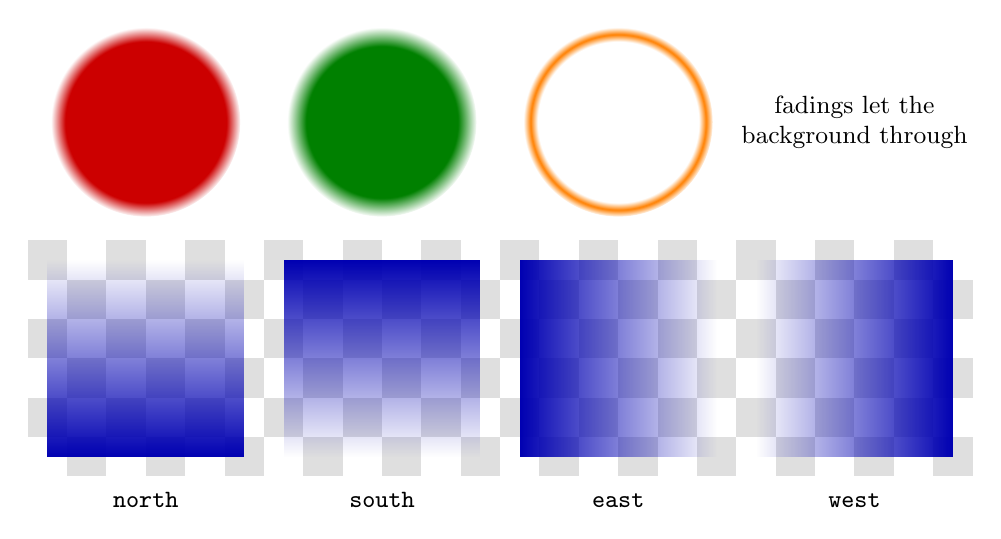
\begin{tikzpicture}
  % a checkerboard behind shows how much of each fill fades away
  \foreach \x in {0,...,23} \foreach \y in {0,...,5} {
    \pgfmathtruncatemacro\k{mod(\x+\y,2)*25}
    \fill[gray!\k] (\x*0.5,\y*0.5) rectangle +(0.5,0.5);
  }
  \foreach \f [count=\i from 0] in {north, south, east, west} {
    \fill[blue!70!black, path fading=\f] (\i*3+0.25,0.25) rectangle +(2.5,2.5);
    \node[fill=white, font=\small\ttfamily, inner sep=1pt] at (\i*3+1.5,-0.3) {\f};
  }
  \fill[red!80!black, path fading=circle with fuzzy edge 15 percent] (1.5,4.5) circle (1.2);
  \fill[green!50!black, path fading=circle with fuzzy edge 20 percent] (4.5,4.5) circle (1.2);
  \fill[orange, path fading=fuzzy ring 15 percent] (7.5,4.5) circle (1.2);
  \node[fill=white, font=\small, inner sep=1pt, align=center] at (10.5,4.5) {fadings let the\\background through};
\end{tikzpicture}
